% The final version needs to be converted to word (or other related format)
% so there's no point in spending a huge amount of time getting everything
% looking perfect in this document.  But it will be much easier for us to
% collaborate with latex rather than word.
%
% Pages 10-15
% Due: 31 Dec 08 !!
% 
% Want lots of graphics and illustrative code samples
% All graphics need to work in black & white


\documentclass[oneside]{article}
\usepackage{fullpage}
\usepackage[pdftex]{graphicx}
\graphicspath{{graphics/}}
\DeclareGraphicsExtensions{.png,.pdf}
\usepackage{hyperref}
\usepackage{verbatim}
\renewcommand\rmdefault{bch}
\usepackage[small]{caption}
\usepackage[tiny]{titlesec}
\titlelabel{}
\linespread{1.07} 

\usepackage[round,sort&compress,sectionbib]{natbib}
\bibliographystyle{plainnat}

\title{Beautiful data: The housing crisis in CA}
\author{Deborah F. Swayne and Hadley Wickham}
\date{\today}

\raggedbottom

\begin{document}
\maketitle 

\section{Introduction}

Motivation: housing crisis.  Can we use housing sale data to quantify it more accurately?  How do our findings compare to findings reported by the media?  Can we locate market segments that were particularly badly hit?

All data and code is available from our git repository - \url{https://github.com/hadley/sfhousing}.  You can see some of the false starts that we made.  Both code and data are licensed with the MIT license. We'll illustrate snippets of code here: you probably won't be familiar with R, but you should still be able to get the gist of it.  Mention the file name next to each section in which it is used.

\section{How did we get the data?}

Like many of our for fun data explorations, this all started when we discovered an interesting data source: the weekly housing sales data provided by the SF Chronicle (\url{}). We had initially planned on scraping the data off the website, but a little detective work revealed that the data is already available in a machine readable form. 

For each week, there was a text file containing all of the data in the following form:

\begin{verbatim}
rowid: 1
county: Alameda County
city: Alameda
newcity: 1
zip: 94501
street: 1220 Broadway
price: $509,000
br: 4
lsqft: 4420
bsqft: 1834
year: 1910
\end{verbatim}

Each file was available at a url of the form \url{http://www.sfgate.com/c/a/year/month/day/REHS.tbl}.  We used R to generate a sequence of Sunday's from the first on record, 2003-04-27, which we found with a little more detective work, to the most recent.  With those dates in hand, we made a list of all the urls and then used the command line tool {\tt wget} to download them all.   We used wget because of it's support for resuming where it left off.  If our internet connection went down or we moved our laptop to another network we didn't need to worry about starting for scratch.  Saves a lot of time!

The next step was to get the data into a more standard format: we chose csv because each file had (approximately) the same fields, and it's a format that all statistical packages (and excel etc) can import and export.  This isn't a standard data format, but nevertheless it's fairly easy to write a parser to deal with it.  This gives us a file like follows:

\begin{verbatim}
county,city,zip,street,price,br,lsqft,bsqft,year,date,datesold
Alameda County,Alameda,94501,1220 Broadway,509000,4,4420,1834,1910,2003-04-27,NA
Alameda County,Alameda,94501,429 Fair Haven Road,504000,4,6300,1411,1964,2003-04
-27,NA
Alameda County,Alameda,94501,2804 Fernside Boulevard,526000,2,4000,1272,1941,200
3-04-27,NA
Alameda County,Alameda,94501,1316 Grove Street,637000,3,2700,1168,1910,2003-04-2
7,NA
\end{verbatim}

This is a little less human readable, but it's a very standard format that practically any tool can read in.  Another minor advantage of this more compact form (not repeating the field names all the time) was reduced storage requirements: 88 vs 45 meg.  Note that R uses {\tt NA} to represent missing values.

Takes just a few minutes to parse all 293 data files.  But a few hours tweaking the parser to get all the edge cases.  Things like stripping \$ and , out of prices to get a number.  And parsing the sold dates, which weren't in a totally consistent format.

Total of 521,726 records.  Had to update mid-way throughout analysis procedure to get the latest data.  This is where having a well though-out script really helps.  Very common in real-life statistical analysis: data is always changing because new data is collected, or old data is corrected.  

\section{Geocoding} 

How to geocode 400,000 addresses?  

Web services - google, yahoo - restrictive licensing clauses.

UCGS.  How long it look to geocode them all.  Send paragraph to Dan Goldberg to check for accuracy.  Never hurts to spend a lot of time checking the data at this level as everything else depends on it.  However, will omit a lot of the work we did because it's more interesting to talk about the findings.

Bar chart showing address quality.  Make sure to have percent on the y-axis.  Won't throw out bad matches right away, because we need varying levels of accuracy for different purposes: city level accuracy is fine when we are comparing cities, will want address level when we are looking within a city, or focusing on purely geographical comparisons.

%       QUALITY_ADDRESS_RANGE_INTERPOLATION 75.30\%
%             QUALITY_EXACT_PARCEL_CENTROID  9.85\%
% QUALITY_ZIP_CODE_TABULATION_AREA_CENTROID  7.11\%
%       QUALITY_COUNTY_SUBDIVISION_CENTROID  0.12\%
%         QUALITY_UNIFORM_LOT_INTERPOLATION  0.04\%


\section{Analysis}

We'll start by looking at number of sales and average prices over all of California, and then zoom into focus on regions of interest.  Finally, we'll look at a few plots that reveal features of the data that allow us to investigate other housing patterns in California.

\begin{figure}[htbp]
  \centering
    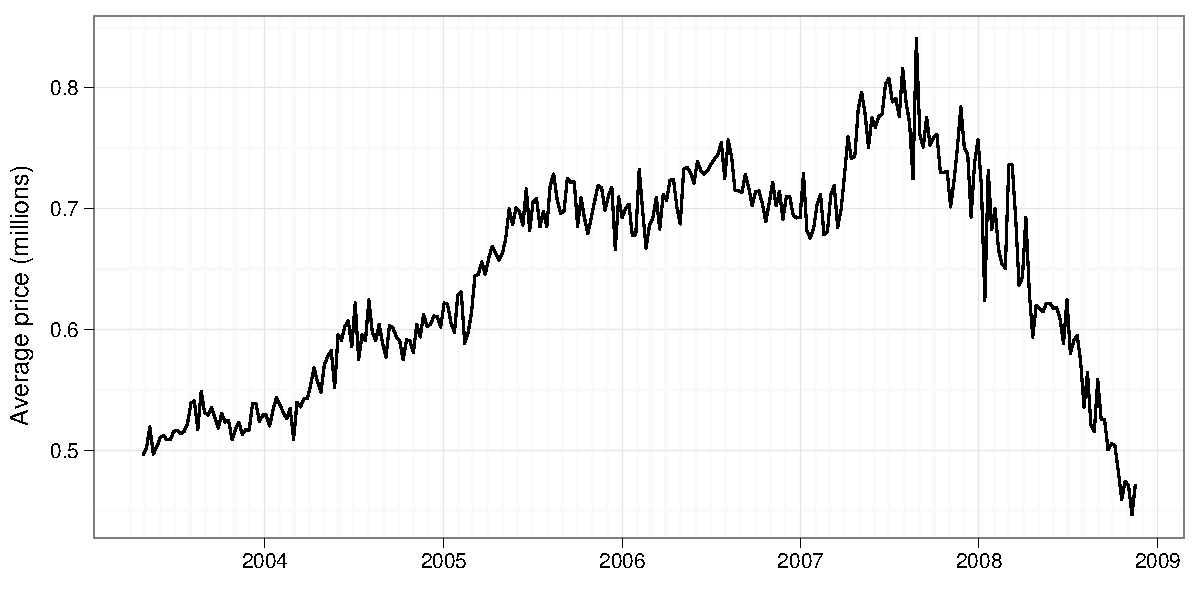
\includegraphics[width=0.5 \linewidth]{daily-price}%
    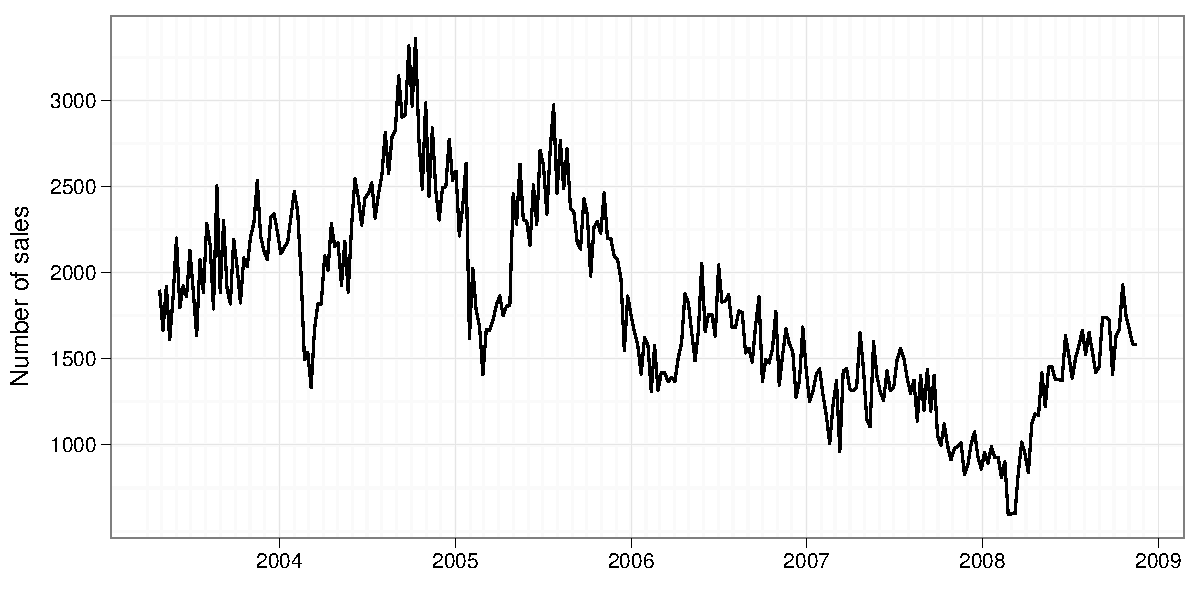
\includegraphics[width=0.5 \linewidth]{daily-sales}
  \caption{Daily average prices (right) and sales (left)}
  \label{fig:daily}
\end{figure}

Figure~\ref{fig:daily} shows average daily sales and prices over the course of the data.  The effect of the housing crisis is striking in the average sale prices, with an increasing trend until June 2007 and then a rapid decrease.  Sales show a different pattern.  We see a gradual decrease in number of sales from mid 2006, and then an increasing trend in early 2008. Maybe this is because of people buying foreclosed houses?  We'll look at that in more detail later on.

\subsection{Adjusting for inflation}

CPI data - \url{http://www.bls.gov/CPI}.  This is a common theme in data analysis: we need to combine our original data with new data that provides context and helps us understand it better.  In this case, we want to control for changes in relative buying power (i.e.\ inflation).  Even over this relatively short time span it's a bad idea to ignore inflation: \$1\,000 2004 dollars would be worth\$1\,170 today.

We used the CPI time series for the West coast.  Series name.

To compute a measure of inflation, we index this time series at the first date in the data.  Indexing means we divide all of the values by the first value: this converts the values into proportions, which makes it easy to read the effect of inflation from the graph.  A value of 1.1 represent a cumulative inflation of 10\% from the start of the data.  Indexing is a very useful technique and we'll use it throughout this chapter.

Figure~\ref{fig:inflation} shows the CPI-based inflation measurement and the affected of adjusting for inflation.  Failing to adjust for inflation makes the increasing trend prior to mid 2007 look more pronounced.  All prices in the remainder of this paper will be inflation adjusted.

\begin{figure}[htbp]
  \centering
    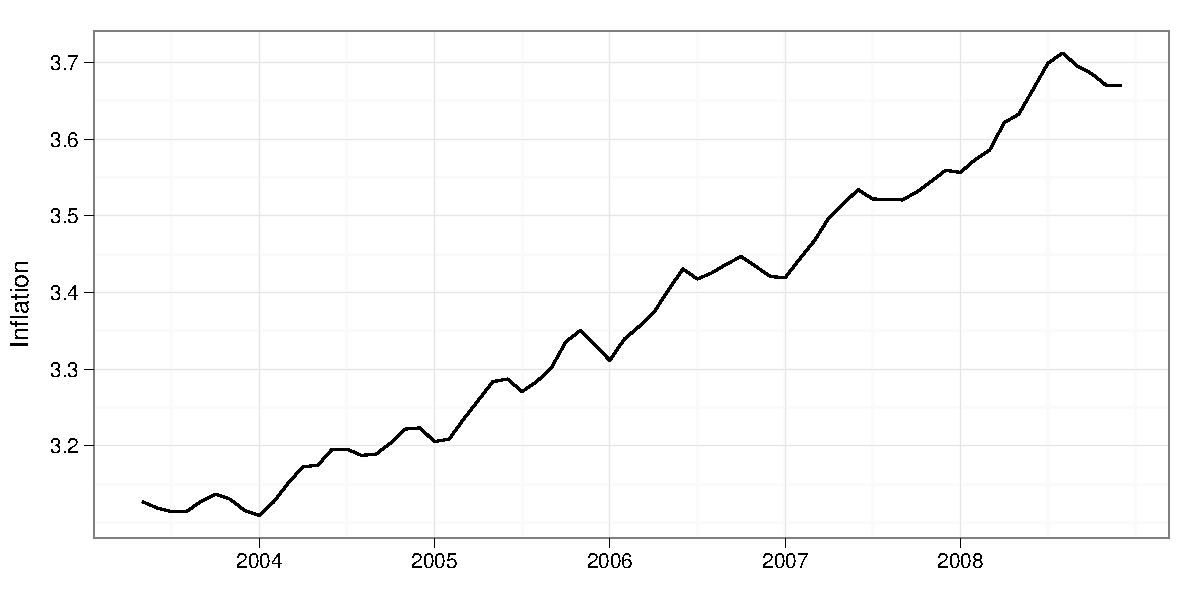
\includegraphics[width=0.5 \linewidth]{daily-cpi}%
    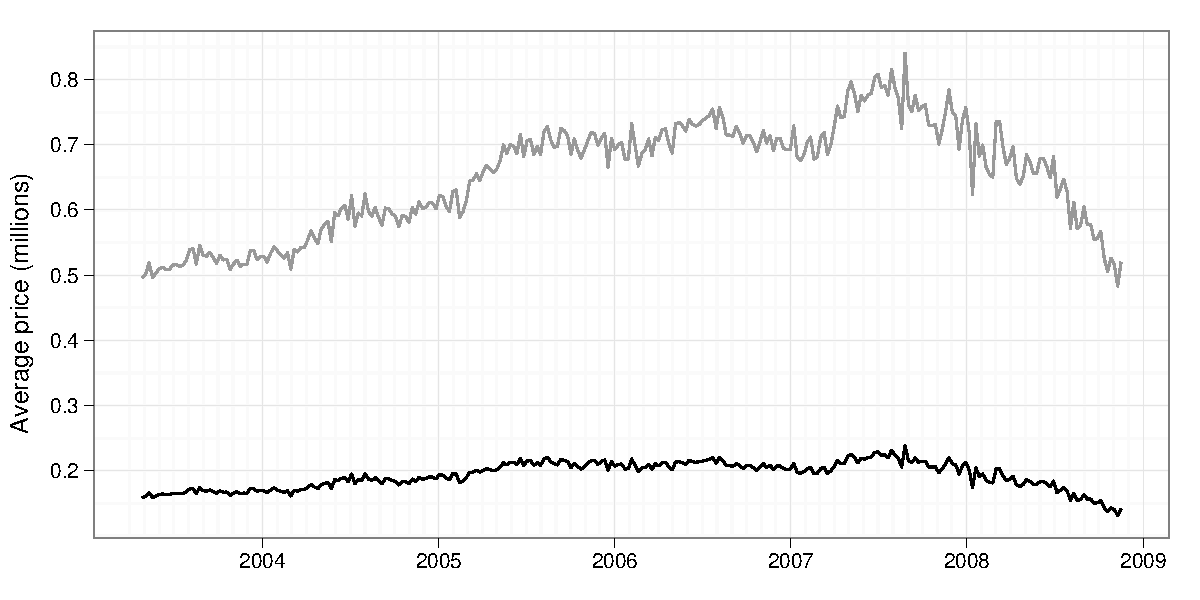
\includegraphics[width=0.5 \linewidth]{daily-price-adj}
  \caption{(Left) Inflation, indexed at 1 at start of series.  (Right) Inflation adjusted prices (black), and unadjusted prices (grey).  Failing to adjusting for inflation makes the rise look steeper, but has little effect on the decline.}
  \label{fig:inflation}
\end{figure}

\subsection{The rich get richer and the poor get poorer}
% explore-deciles.r

We were also interested to investigate whether the housing crisis has equally affect the rich (people owning the most expensive houses) and the poor (the people only the least expensive houses).  To explore this, for each month of sales, we calculate price deciles.  The deciles are the nine numbers that split the price into ten bins each containing the same number of houses,  from least expensive to most expensive.  For example, ...

Figure~\ref{fig:decile-raw} shows how the deciles have changed over time.  The top line is the number that 90\% of houses are less than, and the bottom line represents the price that 10\% of houses are cheaper than.  We can see the effect of the housing bubble in mid 2007, particularly in the most expensive houses.  However, it's probably better to look at the indexed values, as in Figure~\ref{fig:decile-index}.  Here we see that the cheaper houses peaked earlier and had a much sharper drop.  The cheapest houses lost 43\% of their value compared to only 9\% for the most expensive houses.

\begin{figure}[htbp]
  \centering
  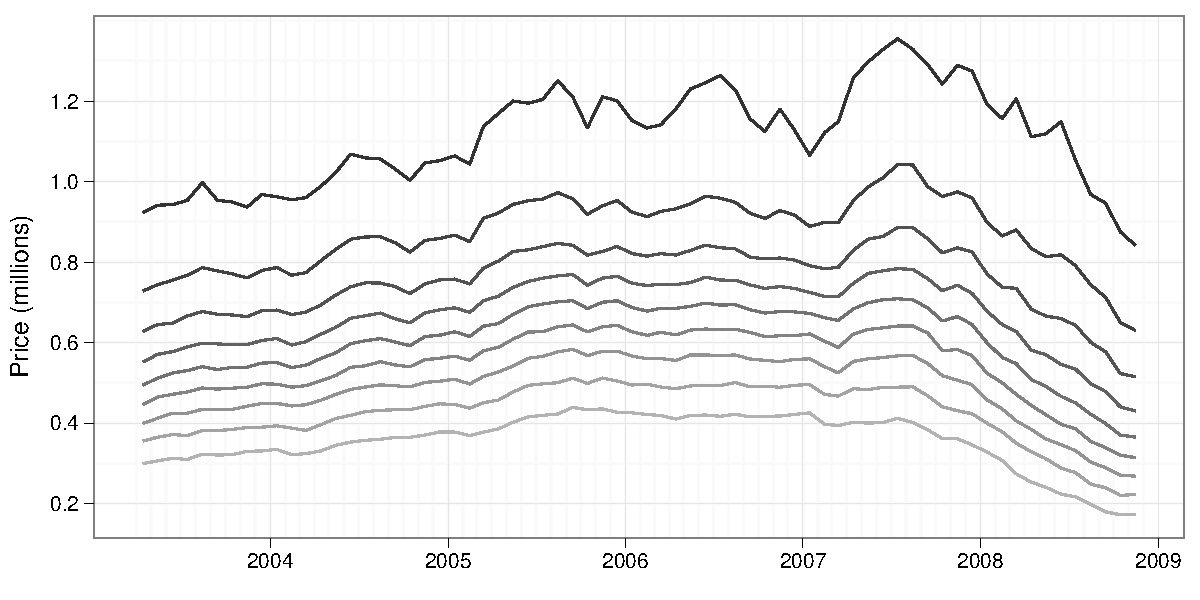
\includegraphics[width=0.75\linewidth]{decile-raw}
  \caption{Average house price within each decile.  Cheaper houses (lower deciles) are coloured lighter.} 
  \label{fig:decile-raw}
\end{figure}

\begin{figure}[htbp]
  \centering
  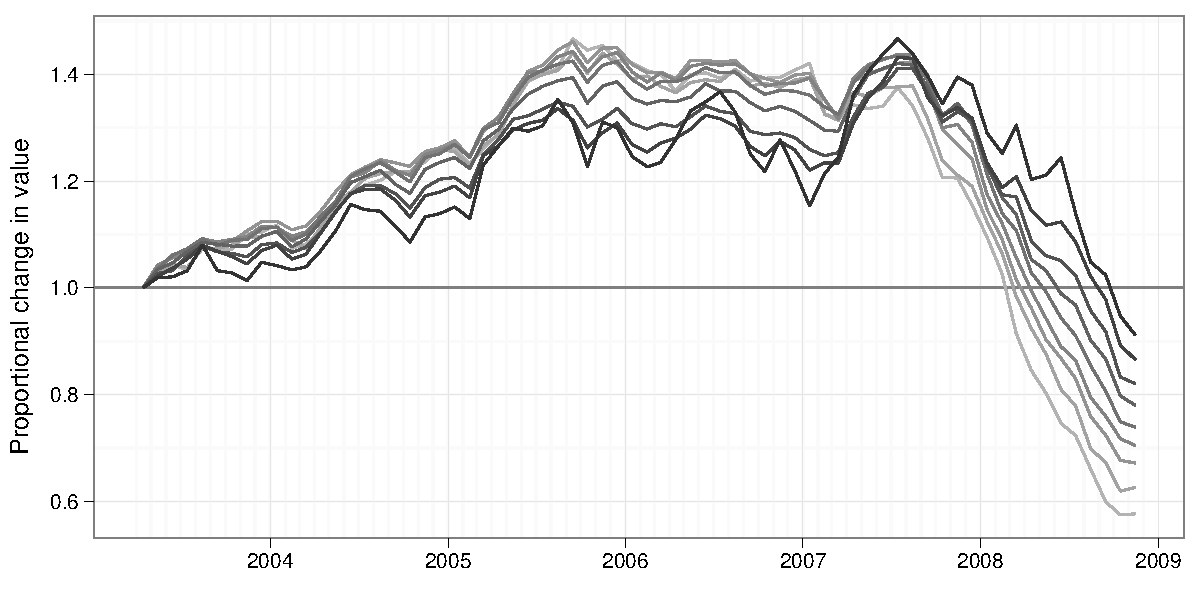
\includegraphics[width=0.75\linewidth]{decile-ind}
  \caption{Indexed house price within each decile.  The average price of cheaper houses increased more rapidly, and fell to much lower lows.}
  \label{fig:decile-ind}
\end{figure}

Another way to look at this inequality is Figure~\ref{decile-rel}.  Here we have standardised the price of an ``average'' home to one.  Relative to an average home, expensive houses have been getting more expensive and cheap houses cheaper.

\begin{figure}[htbp]
  \centering
  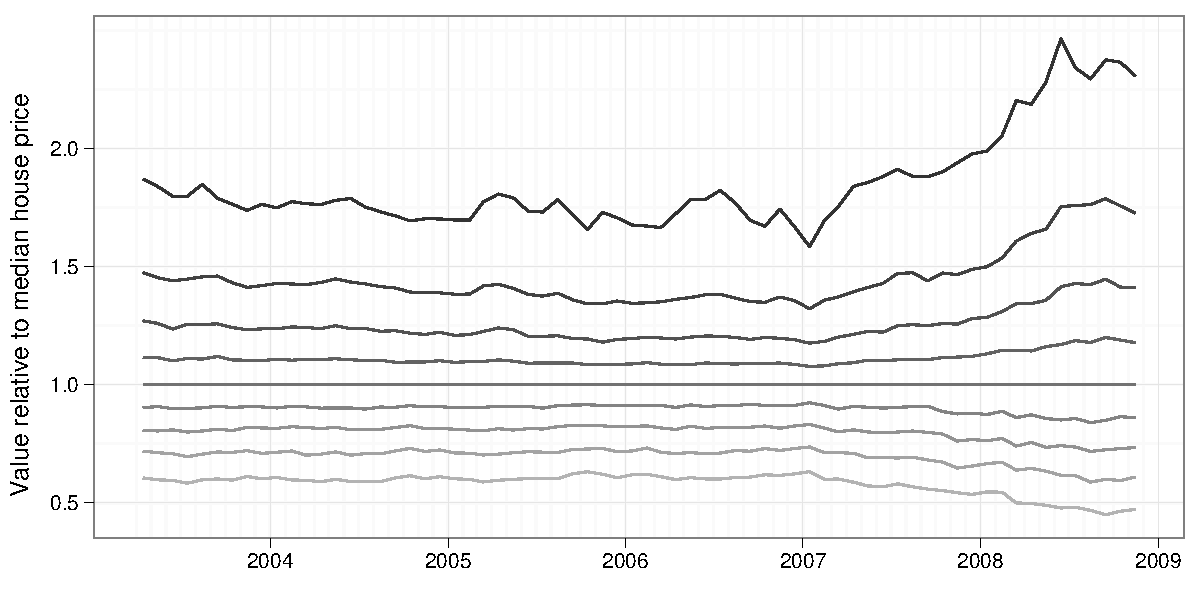
\includegraphics[width=0.75\linewidth]{decile-rel}
  \caption{House prices, relative to the price of the median priced home.  The disparity in home prices is increasing.}
  \label{fig:decile-rel}
\end{figure}

\subsection{Geographic differences}

% See explore-city.r for code.

Big city level break down: chose all cities with more than 2910 sales in total, an average of 10 sales per week.  Gives us 59 cities in California with a total of 423,527 (out of an original 521,726, 81\% of the original data).  

% Figure~\ref{fig:big-cities} shows the counts for the 20 biggest cities.
% 
% \begin{figure}[htbp]
%   \centering
%   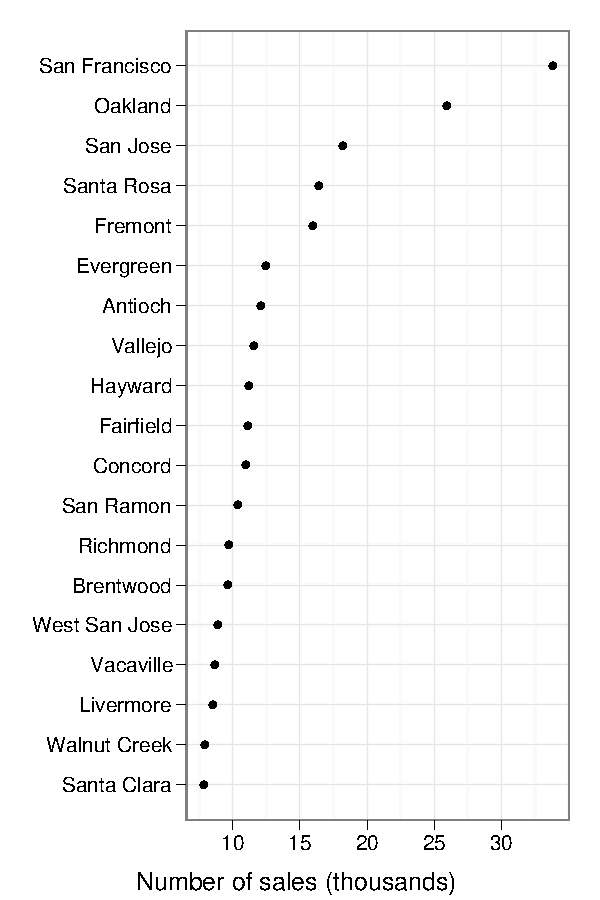
\includegraphics[width=0.5\linewidth]{big-cities}
%   \caption{Total housing sales for the 20 biggest cities.}
%   \label{fig:big-cities}
% \end{figure}

From this reduced data we then calculated the number of sales and the average sale price for each city for each week.  Figure~\ref{fig:spaghetti} shows this data, with each city as a different line.  Statisticians have an evocative name for this type of plot: the spaghetti plot.  It's very hard to see anything in the big jumble of lines.  We're going to use two techniques to bring some order to the mess.  First, we're going to smooth the lines to focus on the overall trend, removing short-term variation that we're not so interested in.  Next, we'll attempt to cluster the cities in groups that show similar patterns.

\begin{figure}[htbp]
  \centering
    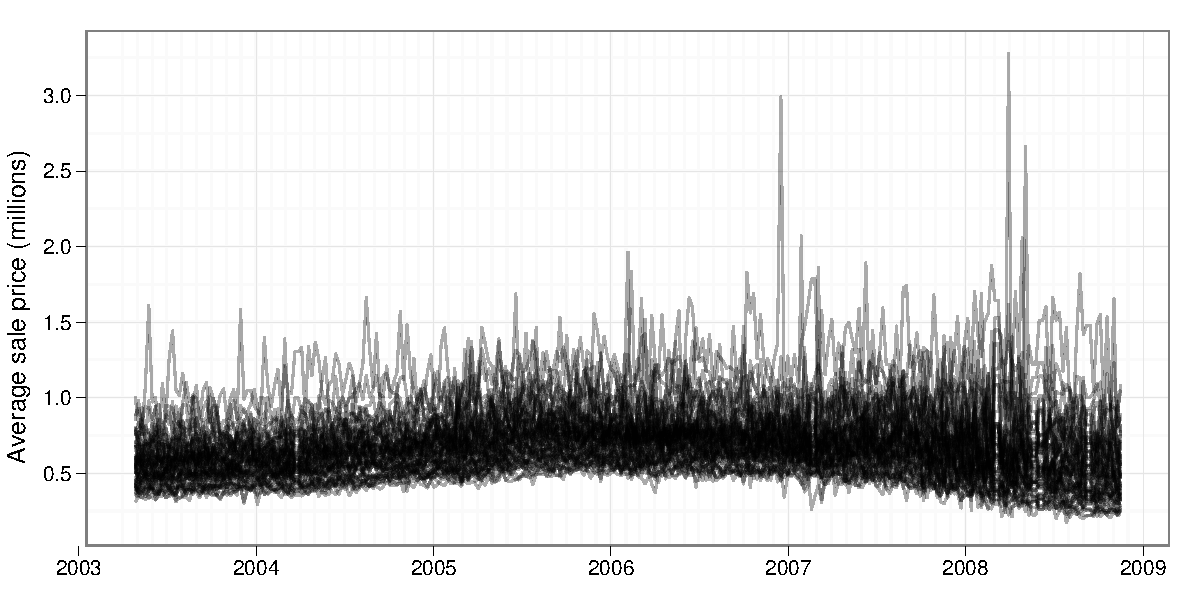
\includegraphics[width=\linewidth]{cities-price}
  \caption{Average sale price for each week for each city.  This type of plot is often called a spaghetti plot for obvious reasons}
  \label{fig:spaghetti}
\end{figure}

Generalised additive models ({\sc gam}) are a generalisation of linear models \citep{wood:2006}.  A linear model has the basic form $y = a + b * x$, and {\sc gam}s generalise this to $y = f(x)$ where x is a smooth line.  A linear model is special case of a {\sc gam} because lines are very smooth functions!  Thin plate regression splines.  We define wiggliness by the second derivative and then penalise it: the final result is a compromise between fit and wiggliness.

But don't worry if you don't understand the details: the gist is that {\sc gam}s are a useful way of removing noisy short-term effects and focussing on the general smooth trend.  This is what we want: for this investigation, we're not interested in changes from week to week or day to day, we're interested in exploring the long term changes related to the housing crisis.

Displaying the smooth curves is an improvement, as in Figure~\ref{fig:smoothed}.  Note the big difference in scales: smoothing the data has removed the very large spikes which represent the sales of very expensive houses.  But there are still a lot of the lines in that plot and we might be missing important findings.  We'll make one other change to the data, we'll index each city: this removes the overall average price of the city and put's it onto an interpretable scale: proportional change in price since the start of the data.  

Instead of displaying them all together, we display each city on a separate plot, as in Figure~\ref{fig:individual}.  This takes up a lot of room, but if you have a big screen or a good printer it's very worthwhile.  We can pick out some interesting patterns: San Francisco, Berkeley and Mountain view all show less of a peak and less of a drop: are more valuable than in 2004.  Other cities show big peaks and big drops: Oakley, Vallejo, and San Pablo.

\begin{figure}[htbp]
  \centering
  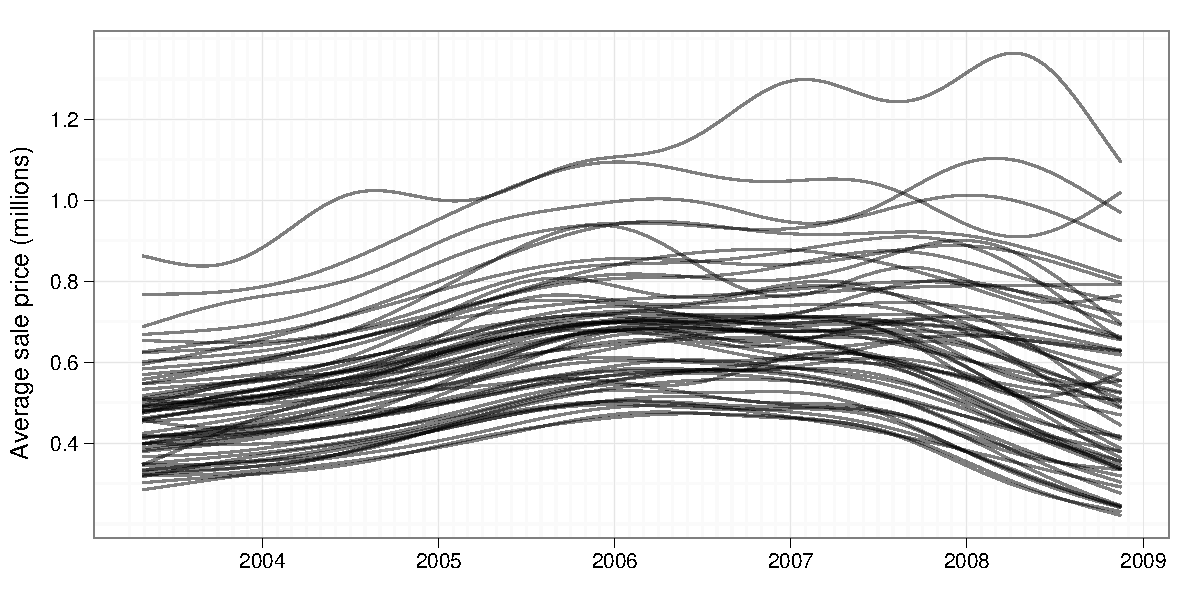
\includegraphics[width=0.5 \linewidth]{cities-smooth}%
  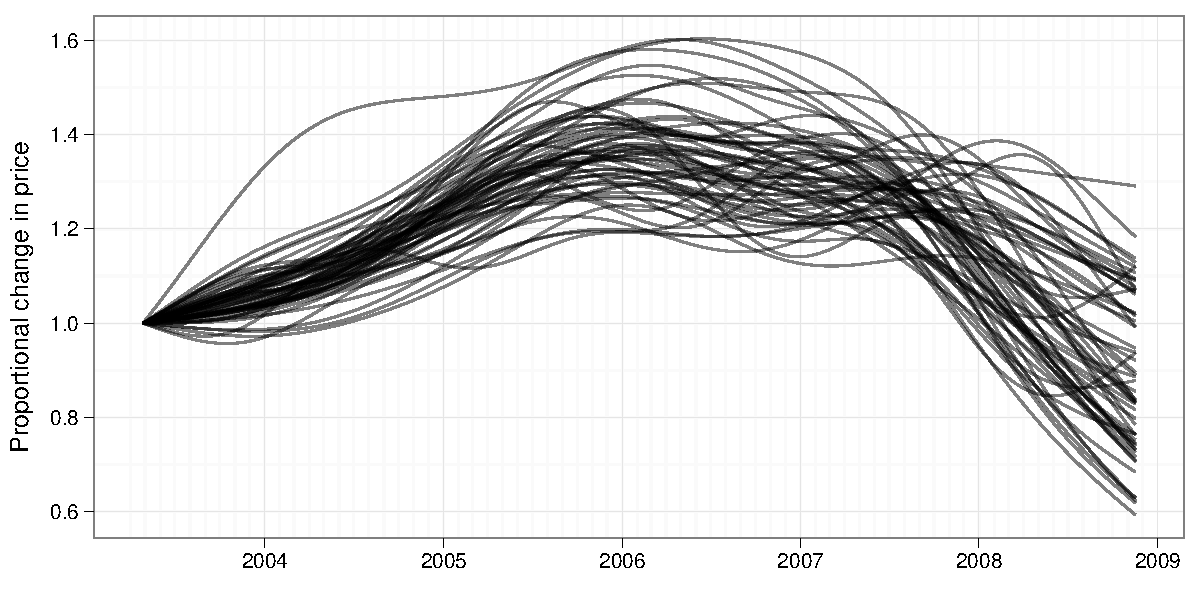
\includegraphics[width=0.5 \linewidth]{cities-indexed}
  \caption{Smoothed city-level weekly average sale prices.  Compared to the non-smoothed version it's easier to see the long-term trends, but it's still not particularly easy}
  \label{fig:smoothed}
\end{figure}

\begin{figure}[htbp]
  \centering
  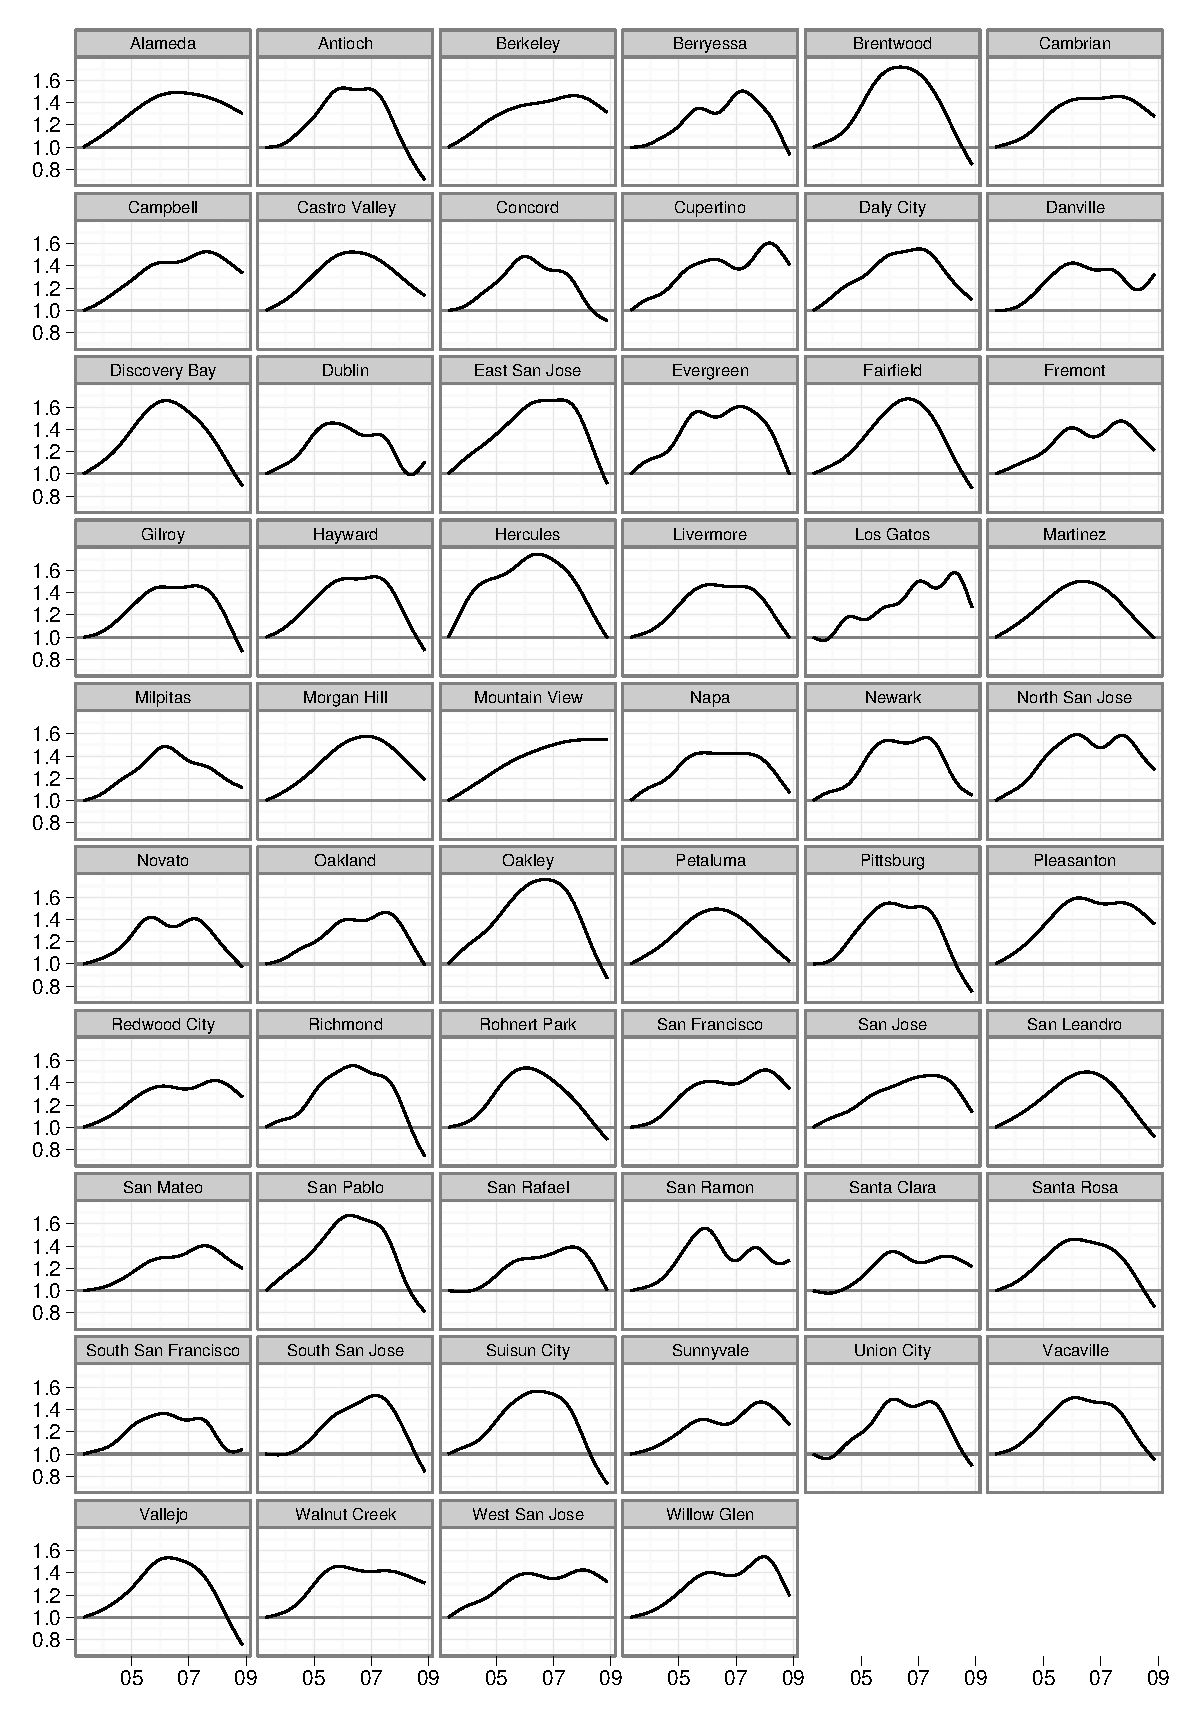
\includegraphics[width=0.9 \linewidth]{cities-individual}
  \caption{Individual plots for each city.  Axis labels have been removed to save space, but the same limits are used for each plot.}
  \label{fig:individual}
\end{figure}

After a few false starts we released that there were two main features that seemed to distinguish the different cities: the height of the peak in the boom and the most recent plummet.  Figure~\ref{fig:clustering} shows one way of clustering the cities into three groups.  Note how the groups are basically formed along the diagonal: it's the difference between the peak and the plummet that seems to be telling us the most.  Figure~\ref{fig:clustered} shows the result of the clustering, with each of the three groups displayed in its own panel.  The groups are somewhat arbitrary (we could shift the boundaries a little in either direction and have little effect)

\begin{figure}[htbp]
  \centering
    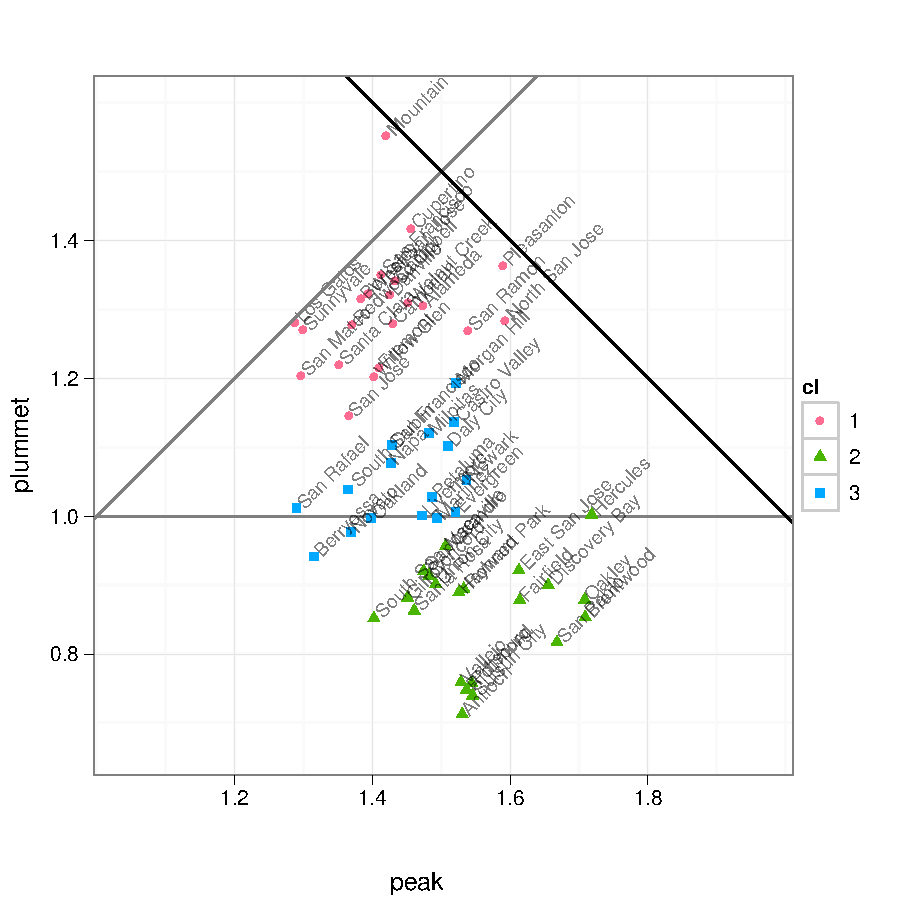
\includegraphics[width=0.7 \linewidth]{cities-clustering}
  \caption{A scatterplot of cities with height at peak on x axis, and most recent value (plummet) on y axis.  The cities have been clustered into three groups.  The closer a city is to the line in the top left corner, the less the effect of the housing crisis on average prices.}
  \label{fig:clustering}
\end{figure}

\begin{figure}[htbp]
  \centering
  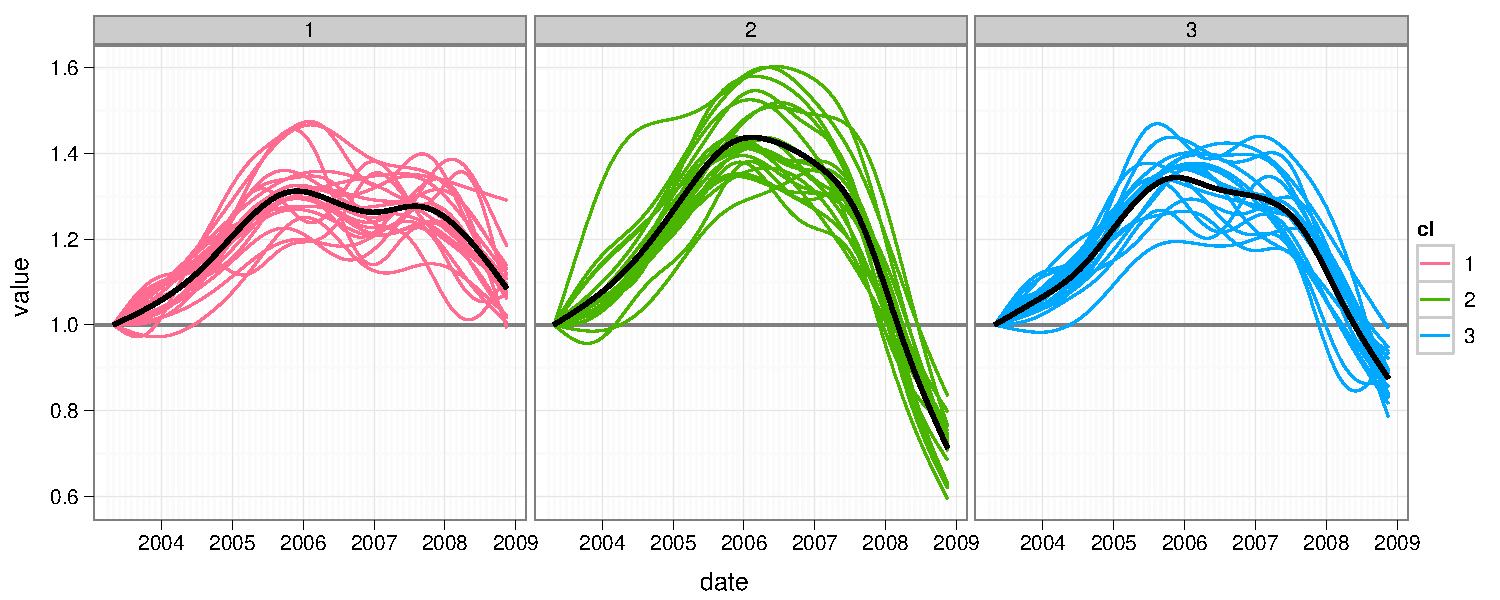
\includegraphics[width=\linewidth]{cities-indexed-clustered}
  \caption{The index sale price time series for the three clustered identified in Figure~\ref{fig:clustering}.  Cluster one includes cities with low peak and no plummet, cluster two cities with high peak and big plummet, and cluster three is somewhere in between.  The thick lines represent smoothed patterns within each cluster.}
  \label{fig:clustered}
\end{figure}

\section{Watching city growth}

We can also use this data for an unexpected purpose.  Because the data is so dense and includes the year that the house was built, we can explore historical patterns of housing development.  This idea was inspired by truliaHindsight, \url{http://hindsight.trulia.com/}, but because we have the data in an unencumbered form we are much freer to experiment with the visualisation of this data.  They have much more data, 150,000 vs 27,000, but we can display more (they display at most 2000 points at once), and we can do more sophisticated analyses.

We'll overlay the data on a map of San Francisco from openstreetmap.

Histogram of year built.

You can see features like golden gate park and so on.

\section{Conclusions}

All the tools we use are open source: you can download them and replicate our work yourselves.  The principle of reproducible research (cite Gentleman and Temple Lang) paper is very important for science - we provide enough detail that you can follow out work every step of the way, and you can run a script to reproduce exactly what we did.  A little tricky because working on this data analysis also lead us to develop some new tools, and it takes some time for these to trickle into released versions.  If you have problems running the code we released, please let us know!  Data analysis like software development.  Local caches to speed things up and to provide some backup if the original sources go down.

Tension with interactive tools: they are great for discovery, but bad for reproducibility.  Once you have discovered something in your interactive tool, you need to be able to reproduce it independently so that others can see it too.  Area of active research (cite Heer's work).  Also need to note your findings as you go along - no way to do this purely in code.  If you read the code on the website you'll see we've used comments to note down what we see and the analysis follows a fairly logical flow.  This is different to what happens in practice - there are many blind alleys that didn't make the final cut.  We rely on the rcs system to keep these, although currently lacking tools to easily search past versions and see the wrong paths that we went down.

Tools: shell (wget, awk); R (ggplot2, plyr, reshape).

Note about graphics: can churn out rough versions for exploration very quickly - takes more time to polish them for publication.  Clarify story, remove extraneous elements and ensure that it supports the text.


% bibtool -x beautiful-data.aux > references.bib
\bibliography{references}

\end{document}
